\documentclass[10pt]{beamer}
 
\usetheme[sectionpage=none, subsectionpage=none, progressbar=none]{metropolis}           % Use metropolis theme
 
  \usepackage{outlines}
  \usepackage{caption}
  \usepackage{appendixnumberbeamer}
  \usepackage{booktabs}
  \usepackage{tcolorbox}
  \usepackage{tabularx}
  \usepackage[export]{adjustbox}[2011/08/13]
  \usepackage{bm}

\newcolumntype{R}{>{\raggedleft\arraybackslash}X} 

\newtheorem*{defn}{Def'n}

  
 \setbeamertemplate{footline}[frame number]{}

\setbeamertemplate{footline}{% 
  \hfill% 
  \usebeamercolor[fg]{page number in head/foot}% 
  \usebeamerfont{page number in head/foot}% 
  \insertframenumber%
  %\,/\,\inserttotalframenumber
  \kern1em\vskip2pt% 
}

\makeatletter
\setbeamertemplate{headline}{%
  \begin{beamercolorbox}[colsep=1.5pt]{upper separation line head}
  \end{beamercolorbox}
  \begin{beamercolorbox}{section in head/foot}
    \vskip2pt\insertnavigation{\paperwidth}\vskip2pt
  \end{beamercolorbox}%
  \begin{beamercolorbox}[colsep=1.5pt]{lower separation line head}
  \end{beamercolorbox}
}
\let\@@magyar@captionfix\relax % IMPORTANT: This is a workaround to fix a random eror with the 2018 installation
\makeatother

\usepackage{xcolor} 
\listfiles

\setbeamercolor{section in head/foot}{fg=normal text.bg, bg=structure.fg}

    \usepackage{smartdiagram}
    \usepackage{tikz}
\usetikzlibrary{shapes.geometric, arrows}
\tikzstyle{startstop} = [rectangle, rounded corners, minimum width=3cm, minimum height=1cm,text centered, draw=black, fill=red!30]
\tikzstyle{io} = [trapezium, trapezium left angle=70, trapezium right angle=110, minimum width=3cm, minimum height=1cm, text centered, draw=black, fill=blue!30]
\tikzstyle{process} = [rectangle, minimum width=3cm, minimum height=1cm, text centered, draw=black, fill=orange!30]
\tikzstyle{decision} = [diamond, minimum width=3cm, minimum height=1cm, text centered, draw=black, fill=green!30]

\title{Gov 2006: Formal Political Theory II \\
Section 5}
\date{\today}
\author{ \textbf{Sophie Hill}}


\begin{document}
  \maketitle
  

%%%%%%%%%%%%%%%%%%%%%%%%%%%%%%%%%%%%%%%%%%
\begin{frame}

\frametitle{Today}

\Large
Models of electoral accountability + applications

\begin{itemize}
\item Review: PSET 4, Q2
\item Review: Perfect Bayesian Equilibrium
\item Sanctioning vs. selection \alert{(Fearon, 1999)}
\item Empirical application \alert{(Ferraz \& Finan, 2011)}
\end{itemize}


\end{frame}
%%%%%%%%%%%%%%%%%%%%%%%%%%%%%%%%%%%%%%%%%%
\begin{frame}{PSET 4, Q2}

\textbf{Q2 (a)} Show that no pooling equilibrium exists if voters won't re-elect politicians when types are not revealed.

\begin{figure}
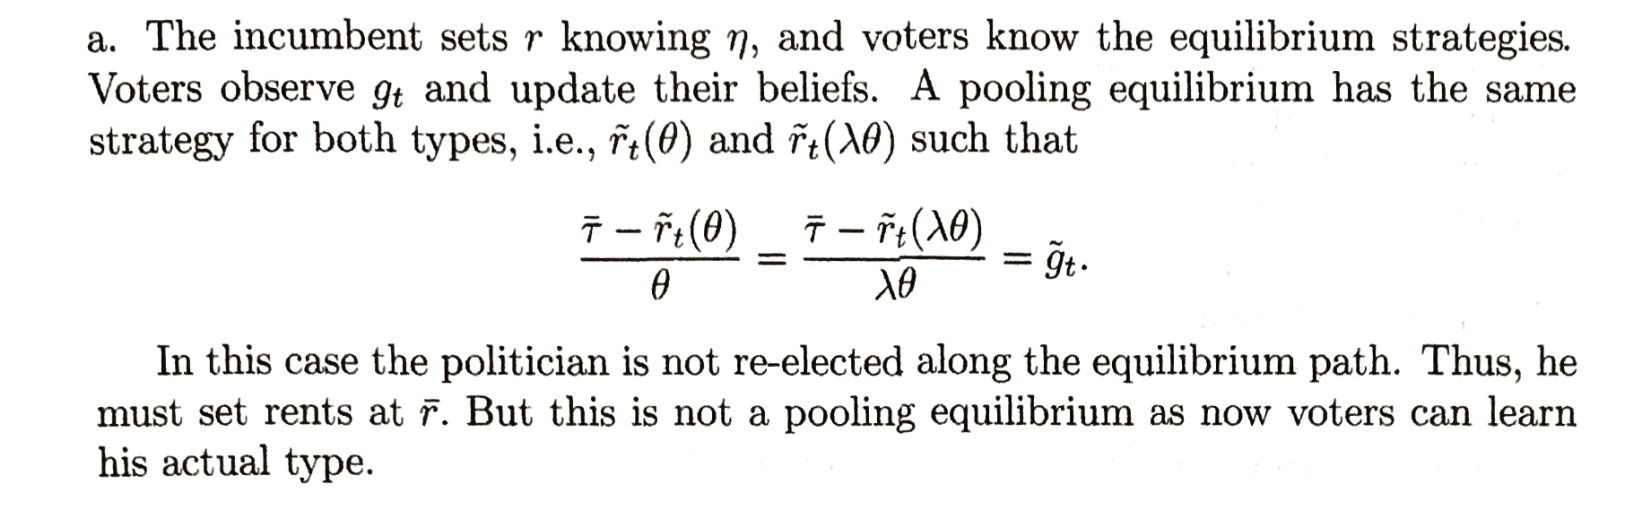
\includegraphics[width=\textwidth]{q21.png}
\end{figure}


\end{frame}
%%%%%%%%%%%%%%%%%%%%%%%%%%%%%%%%%%%%%%%%%%
\begin{frame}{PSET 4, Q2}

\textbf{Q2 (b)} Now assume that voters may re-elect even if types are not revealed. Show that pooling equilibria exist and survive the weakly dominated strategies refinement.


\begin{figure}
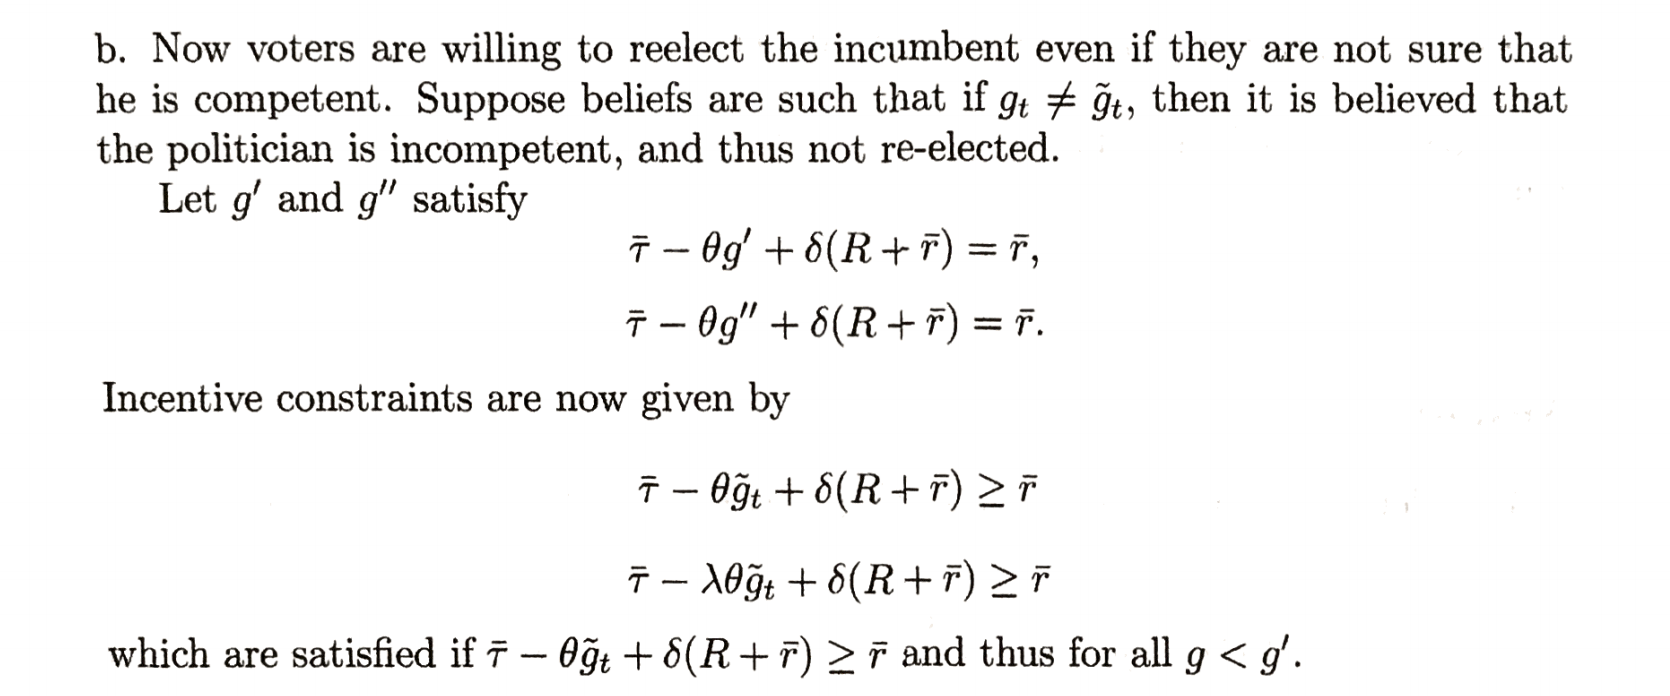
\includegraphics[width=\textwidth]{q22.png}
\end{figure}


\end{frame}
%%%%%%%%%%%%%%%%%%%%%%%%%%%%%%%%%%%%%%%%%%
\begin{frame}{PSET 4, Q2}

\begin{figure}
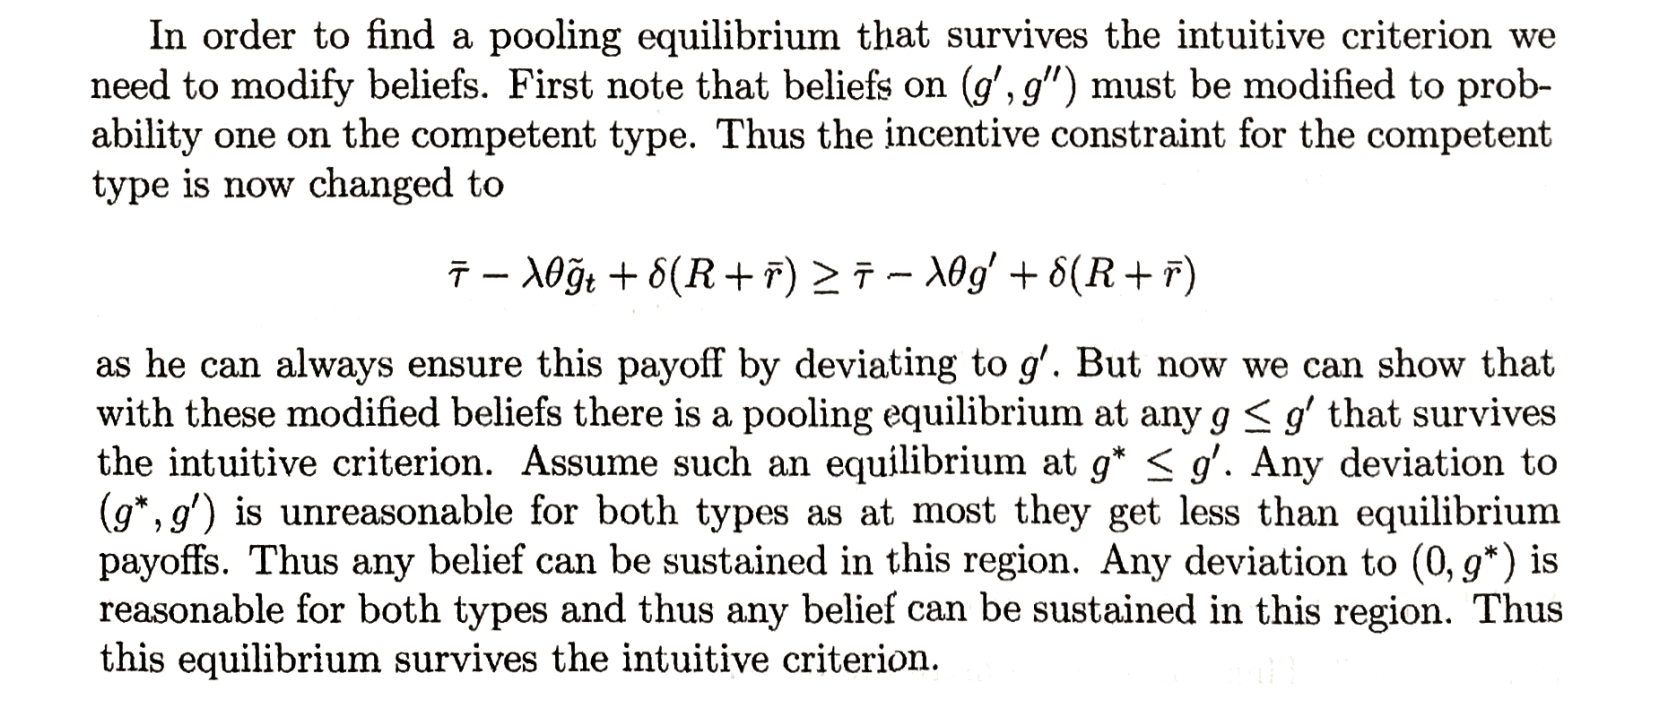
\includegraphics[width=\textwidth]{q23.png}
\end{figure}


\end{frame}


%%%%%%%%%%%%%%%%%%%%%%%%%%%%%%%%%%%%%%%%%%

\begin{frame}{Review: Perfect Bayesian Equilibrium}

\begin{itemize}
\item PBE extends the concept of SPNE to games with \textit{incomplete information} \pause 
\item PBE requires us to specify \textit{beliefs} = a conditional distribution over the nodes of information set $h$ that player $i$ is in, $P_i(v | h) \, \, $ for $ v \in h$
\end{itemize}
 
\pause

\begin{tcolorbox}
A PBE consists of a strategy profile for all players + beliefs about the other players' types at all information sets that satisfies:

\begin{enumerate}
\item \textbf{sequential rationality}: at each information set, each
player's strategy specifies optimal actions, given her beliefs and the strategies of the other players 
\item \textbf{consistent beliefs}: given the strategy profile, the beliefs are consistent with Bayes’ rule whenever possible
\end{enumerate}
\end{tcolorbox}

\pause 
\begin{itemize}
\item What does \textbf{``whenever possible''}  in (2) mean?
% By definition, the information sets off the euilibrium path are reached with probability 0. Hence, we cannot apply Bayes' formula to compute the beliefs.
\end{itemize}

\end{frame}
%%%%%%%%%%%%%%%%%%%%%%%%%%%%%%%%%%%%%%%%%%


\begin{frame}

\frametitle{Fearon (1999)}

Two main ideas about elections: sanctioning vs. selection

\pause 

\begin{itemize}
\item \textbf{Sanctioning} induces politicians to choose in the public interest so they retain their jobs. 
\item \textbf{Selection} allows the public to choose leaders who will decide, of their own accord, to act in the public interest. 
\end{itemize}

\bigskip

This paper: 
\begin{itemize}
\item What's optimal when both moral hazard and adverse selection are present?
\item Integrates retrospective + prospective voting models.
\item Selection wins.
\end{itemize}

\end{frame}
%%%%%%%%%%%%%%%%%%%%%%%%%%%%%%%%%%%%%%%%%%


\begin{frame}

\frametitle{Motivation}

Trying to select good types often means kicking out those who turned out to be bad types in office.

$\Rightarrow$ selection looks like sanctioning.

$\Rightarrow$ bad types have incentives to behave like good types. % (see also Rogoff and Sibert 1988; Rogoff 1990). 

\bigskip

Voters seem to understand elections in terms of selection rather than sanctioning: 
\begin{itemize}
\item They dislike ``office seekers''.
\item They dislike term limits, thinking that they restrict the voters' ability to select who they want.
\item They value consistency a lot and dislike ``waffling''.
\end{itemize}
%The model shows why this is the only rational re-election rule.

\end{frame}



\begin{frame}

\frametitle{Setup}

Two periods, two players: electorate (median voter) $E$, and incumbent $I$. 
\begin{itemize}
\item $E$ has ideal point $x=0$, quadratic utility.
\end{itemize}

\bigskip

Timing: \begin{enumerate}

\item $I$ chooses policy $x$. 
\item $E$ does not observe $x$, but observes noisy outcome $z = -x^2 + \varepsilon$ where $\varepsilon$ is a random variable drawn from $F$.
\item $E$ decides whether to re-elect $I$, or draw a random new politician. 
\item In the second period, politician chooses $y$, yielding voters utility $-y^2+\varepsilon'$ (discounted by $\delta\in(0,1)$). 
\end{enumerate}

\bigskip

$F$ is symmetric, strictly unimodal distribution with mean zero. 

\end{frame}

\begin{frame}

\frametitle{Strategies}

Optimal approach for $E$ is to use a cutoff rule such that they re-elect if $z\geq k$. 
\begin{itemize}
\item See Banks \& Sundaram (1996) on the optimality of this.
\item So, problem is really how to formulate $k$ to best motivate or select politicians.
\end{itemize}

\bigskip

This always looks like retrospective voting -- but consider three types of approaches: pure selection, pure sanctioning, and a mixture.

\end{frame}

\begin{frame}

\frametitle{Pure selection}

Share $\alpha\in(0,1)$ are ``good'' types who will implement $x=0$, while $1-\alpha$ are ``bad'' types who can at best implement suboptimal $\hat{x}>0$. 

\bigskip

$E$ updates belief about type and re-elects if the updated belief about $I$, $\alpha(z)$, is greater than a random draw $\alpha$. 

\bigskip

The posterior odds that $I$ is a good type is: $$\frac{\alpha(z)}{1-\alpha(z)} = \frac{\alpha}{1-\alpha}\frac{f(z)}{f(\hat{x}^2+z)},$$ where the first term is the prior odds and the second term is the likelihood ratio (from $\Pr(z|good)$ and $\Pr(z|bad)$).




\end{frame}

\begin{frame}

\frametitle{Re-election rule}

Therefore, re-election ($\alpha(z)\geq \alpha$) implies: $$f(z)\geq f(\hat{x}^2+z).$$ Therefore, $k^*$ solves: $$f(k^*) = f(\hat{x}^2+k^*).$$

If $F$ is unimodal, then $k^*$ is unique (consider the intersection of the pdfs). 

When $F$ is symmetric, $f(k) = f(-k)$, we have: \begin{eqnarray*}
-k^* = \hat{x}^2 + k^* \hspace{20pt}
\Longrightarrow k^* = -\hat{x}^2/2
\end{eqnarray*}

So $k$ increases with competence of bad type, but does not depend on $F$. 

\smallskip

However, better monitoring (i.e. lower variance of $\varepsilon$) increases the probability of re-electing good types = $1-F(k^*)$ 

\end{frame}

\begin{frame}

\frametitle{Pure sanctioning}

All politicians have same type. Assume politicians want to implement $x=1$ with the utility function: $$W - (1-x)^2 + \delta [W - (1-y)^2],$$ where $W>0$. Obviously always choose $y=1$ in period 2.

\bigskip

\begin{itemize}
\item $E$ indifferent between politicians in second period. 
\item But they control the first period. 
\item $E$ does not want to set too high a standard (re-election is too hard), or too low a standard (re-election is too easy). 
\end{itemize}

\end{frame}

\begin{frame}

\frametitle{Re-election rule}

\small 

$E$ designs $k$ to minimize $x$, recognizing that $I$ solves: $$\max_{x} \bigg\{ W - (1-x)^2 + \delta(1-F(x^2+k))W \bigg\},$$ which yields FOC (assuming conditions that satisfy SOC): $$ f(x^2+k) = \frac{1-x}{x}\frac{1}{\delta W}.$$

$E$ minimizes $x$ by maximizing LHS (given RHS is decreasing in $x$). 

Given $F$ is unimodal and has zero mean, $f$ is maximized at $f(0)$. Therefore, $k^*$ solves: $$x(k^*)^2 + k^* = 0.$$ Substituting in the FOC yields: $$k^* = -x^{*2}, x^* = \frac{1}{1 - \delta Wf(0)}.$$ 

How does monitoring capacity affect $x^*$? \pause Higher variance of $F$ (reducing monitoring capacity) reduces control of incumbent.

\end{frame}

\begin{frame}

\frametitle{A mixed model}

Problems with the previous models.
\begin{enumerate}
\item Pure sanctioning allows for no variation in politician preferences. 
\item Pure selection does not allow bad types to behave well. 
\end{enumerate}

So we need a model including both adverse selection and moral hazard. 

\bigskip

Good and bad politicians differ in their policy preferences. 

\begin{itemize}
\item ``Good'' types have per period utility function $W-x^2$, so desire $x=0$. 
\item ``Bad'' types have per period utility function $W-(1-x)^2$, so desire $x=1$. 
\end{itemize}

Voters must now choose between motivating bad types and selecting good types. 

\end{frame}



\begin{frame}

\frametitle{Solving backwards}

We search for a pure strategy PBE. 

\bigskip

What happens in period 2? \pause For all prior histories of play, good types choose $y = 0$ and bad types choose $y = 1$ in period 2. 

\bigskip

In the first period, $I$ chooses $x_b$ if bad and $x_g$ if good. 

\bigskip

$E$ chooses a cutoff rule $z\geq k$, and have belief $\alpha(z)$. Strategy $s = (x_g, x_b, k)$.

%; see Banks and Sundaram (1996) for the optimality of this. 




\end{frame}



\begin{frame}

\frametitle{Re-election rule}

As always, work backwards. In period 2, $E$ keeps incumbent if:

\vspace{-0.5cm}
\begin{align*}
\alpha(z)\cdot 0 + (1-\alpha(z))(-1) &\geq -(1-\alpha) \\
\Leftrightarrow \alpha(z) &\geq \alpha
\end{align*}

$E$ again re-elects if $\alpha(z)\geq \alpha$, where: $$\frac{\alpha(z)}{1-\alpha(z)} = \frac{\alpha}{1-\alpha}\frac{f(x_g^2+z)}{f(x_b^2+z)}.$$ Therefore, $I$ is re-elected if $f(x_g^2+z)\geq f(x_b^2+z)$. 

\bigskip

So, $k^*$ satisfies: $$f(x_g^2+k^*) = f(x_b^2+k^*).$$


\end{frame}


\begin{frame}

\frametitle{Incumbent's first period behavior}

What does $I=b$ do in the first period? \pause Same problem as in the sanctioning model, so: $$ f(x_b^2+k) = \frac{1-x_b}{x_b}\frac{1}{\delta W}.$$ 

What does $I=g$ do? \pause Chooses $x_g=0$. Applying our cutoff rule yields: $$f(k^*) = f(x_b^2+k^*).$$ 

Given properties of $F$, we have $$k^* = -x_b^2/2$$ 

Substituting into $b$'s FOC yields equilibrium $k^*$: $$f(k^*) = \frac{1-\sqrt{-2k^*}}{\sqrt{-2k^*}}\frac{1}{\delta W}.$$ 

%PBE is unique for sufficiently large variance, and is never $x_b=0$ or $x_b=1$. 

For large enough variance, $\exists$ a unique interior solution that approaches $k = -1/2 \implies x_b = 1$ as monitoring worsens -- i.e., total shirking. 


\end{frame}


\begin{frame}

\frametitle{Discussion}

Simple model, but says interesting things.

\bigskip

\textbf{Selection}
\begin{enumerate}
\item If politicians do not vary in type, then voters are indifferent.
\item Introduce \textit{any} variation in types, then it makes sense for the electorate to entirely focus on selecting good types.
\end{enumerate}

\textbf{Commitment}
\begin{enumerate}
\item Electorate can minimise shirking by using the pure sanctioning $k$.
\item But this makes second period selection harder.
%\item So not credible to focus on sanctioning.
\end{enumerate}

%This undermines the bad politician's incentive not to shirk: if the share of good types is not too large voters would actually be better off if they could commit in advance to use the pure sanctioning cutoff.

\textbf{Monitoring}
\begin{itemize}
\item Better able to screen good from bad politicians.
\item But bad types more incentivized to behave as good types.
\end{itemize}

\bigskip

Inverted-U relationship between monitoring ability and selection ability.

\end{frame}

\begin{frame}\frametitle{Consistent with evidence?}

Time-series: ideological shirking of representatives over time, due to the last-period effect for bad types. 

\bigskip

Cross-section: less shirking by longer-serving representatives. 

\bigskip

Model predicts:
\begin{itemize}
\item Politicians shirk at least as much (good types) or more (bad types) in the second term.
\item As a group, second-term politicians shirk less than first-term politicians because selection implies that some bad types are not reelected.
\end{itemize}


\end{frame}

\frame{\frametitle{``Electoral Accountability and Corruption,'' by Ferraz and Finan.}

\begin{itemize}
\item Ferraz and Finan study theoretically and empirically how electoral accountability affects corruption practices by incumbent politicians.
\item Novel measure of corruption that comes from a famous audit program.
\item {\bf Idea:} They compare mayors with reelection incentives
and those without (second term limit is binding).
\item There should be more corruption in the latter.
\item They find that the difference is larger in municipalities with less 
information and where the likelihood of judicial punishment is lower.
\end{itemize}
}

\frame{\frametitle{Simple Model}

\begin{itemize}
\item Consider a two-period model 
\item Two types of politicians: corrupt -$c$- and non-corrupt -$nc$.
\item $\pi$ is the proportion of non-corrupt in the pool of potential candidates.
\item In each period, the elected candidate sets a state-dependent policy $e_t(s_t ,i)$, where 
\begin{itemize}
\item $i \in \left\{ c, nc \right\}$ is the type of elected politicians and 
\item $s_t \in \left\{ 0, 1 \right\}$ is the state of the world at time $t$.
\end{itemize}
\item Each state happens with equal probability.
\item Voters' payoff is $V$ if $e_t = s_t$, and zero otherwise.
\item Non-corrupt politicians set policy to maximize voter's welfare.
\item Corrupt politicians receive a payoff $r_t$ for setting $e_t \neq s_t$ and ego rents $E$.
\item $r_t$ is drawn period from $G(r)$ with mean $\mu$ and support $\left[ 0, R\right]$.
\item Assume $R > \delta (\mu + E) $, where $\delta$ is the discount factor.
\end{itemize}
}

\frame{\frametitle{Timing}

\begin{itemize}
\item Nature picks incumbents and their type.
\item Nature picks the state of the world $s_1 \in \left\{ 0, 1 \right\}$.
\item Corrupt incumbents receive their draw of $r_1$ from $G(r)$.
\item Incumbents pick policies and payoffs are realized.
\item Voters observe their payoffs and decide whether to reelect their incumbents or not.
\item Nature picks the state of the world $s_2 \in \left\{ 0, 1 \right\}$.
\item Corrupt politicians receive their draw of $r_2$ from $G(r)$.
\item Incumbents pick policies and payoffs are realized.
\end{itemize}
}


\frame{\frametitle{Characterization}

\begin{itemize}
\item We focus on Perfect Bayesian Equilibrium.
\item We solve through backward induction.
\item In period 2, absent reelection incentives, each incumbent picks his preferred policy: $e_2(s_2 ,c) =1 - s_2$ and $e_2(s_2 ,nc) =s_2$.
\item Corrupt politicians then receive rents $r_2$.
\item When voting, voters then maximize the chances they get a non-corrupt politician.
\begin{itemize}
\item If they have payoff zero in period 1, they pick another politician.
\item Otherwise, they reelect their incumbent only if the posterior that they are non-corrupt is larger than $\pi$.
\end{itemize}
\end{itemize}
}


\frame{\frametitle{Characterization}

\begin{itemize}
\item Assume an equilibrium where corrupt incumbents that play as honest get reelected in period 1.
\item The posterior that a given incumbent is non-corrupt is as follows
$$ Pr(i=nc | V) = \frac{\pi}{\pi + (1-\pi) Pr(r_1 \le \delta (\mu + E)) } \ge \pi $$
where $Pr(r_1 \le \delta (\mu + E))$ indicates the probability that the rents of being corrupt
are smaller than the gains from pooling with honest politicians to gain reelection.
\item In equilibrium non corrupt politicians always set $s_t = e_t$ and corrupt politicians set $e_2 = 1 - s_2$, and $e_1 = s_1$
if $r_1 \le \delta (\mu + E)$ and $e_1 = 1- s_1$ otherwise.
\end{itemize}
}


\frame{\frametitle{Bringing the model to the data}

\begin{itemize}
\item Denote the fraction of disciplined politicians $\lambda = G( \delta (\mu + E))$.
\item Ferraz and Finan cleverly note that, if the ratio of disciplined politicians is larger than the share of non-corrupt types, $ \frac{\lambda}{1-\lambda} \ge \pi  $,  then rent extraction will, on average be higher in the second period than in the first period
\end{itemize}
$$(1-\pi) (1-\lambda) \int_{r_1 \geq \delta (\mu + E)}^R r dG(r) \leq $$
$$(1-\pi) \lambda \int_{0}^R r dG(r) + (1-\pi) (1-\lambda) (1-\pi) \int_{0}^R r dG(r) $$

\begin{itemize}
\item A sufficient condition is that 
\end{itemize}
$$(1-\pi) (1-\lambda)  \leq (1-\pi) \lambda + (1-\pi) (1-\lambda) (1-\pi) $$
$$ (1-\lambda)  \leq  \lambda +  (1-\lambda) (1-\pi) $$
$$ 0  \leq  \lambda - (1-\lambda) \pi $$
}

\frame{\frametitle{Timeline of Data}
\begin{figure}[h]
\begin{center}
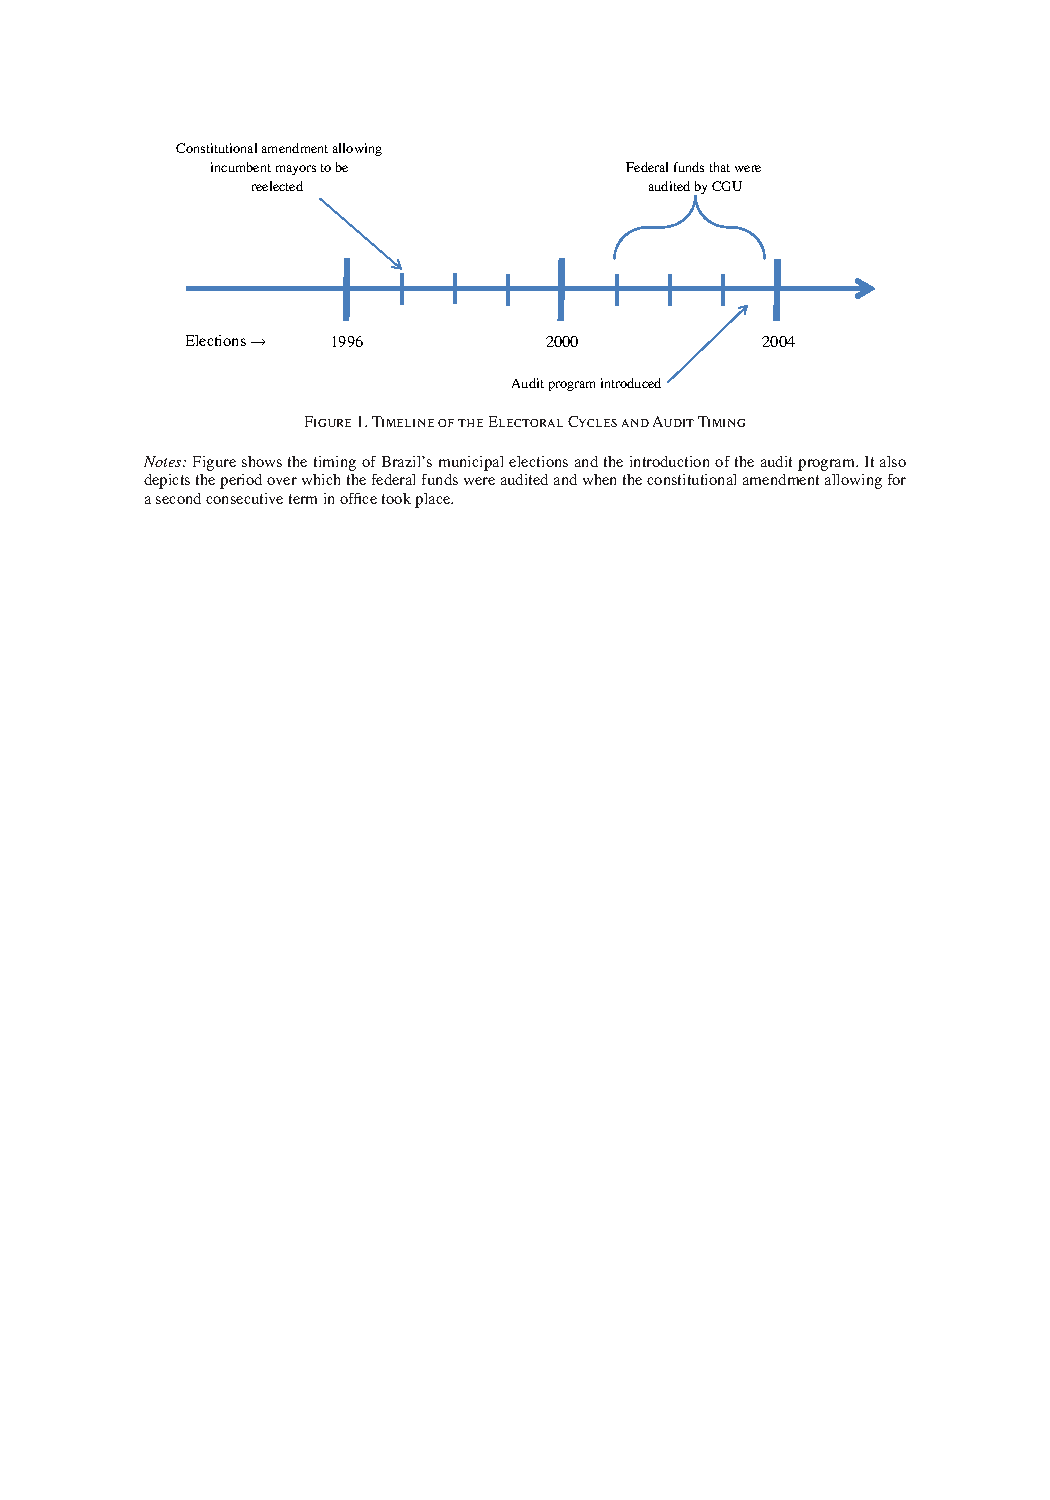
\includegraphics[scale=.8]{Timeline.pdf}
\end{center}
\end{figure}
}

\begin{frame}{Taking the model to the data}

\Large 

\begin{tcolorbox}
How should we bring the comparative static (that corruption rises in period 2) to the data? \alert{What} are we comparing to \alert{what}?
\end{tcolorbox}

\end{frame}

\frame{\frametitle{Potential Issues}

\begin{itemize}

\item Municipalities that have one term mayor and different from those with a second term mayor
\begin{itemize}
\item Perform an regression discontinuity that takes care of that.
\end{itemize}
\item Second term mayor may have better ability.
\begin{itemize}
\item Compare them with first term mayors that then get reelected.
\end{itemize}
\item Second term mayor may have more experience.
\begin{itemize}
\item Add some controls and argue that such a story is inconsistent with their heterogeneous effects.
\end{itemize}
\end{itemize}


}


\frame{\frametitle{Regression Discontinuity}
\begin{figure}[h]
\begin{center}
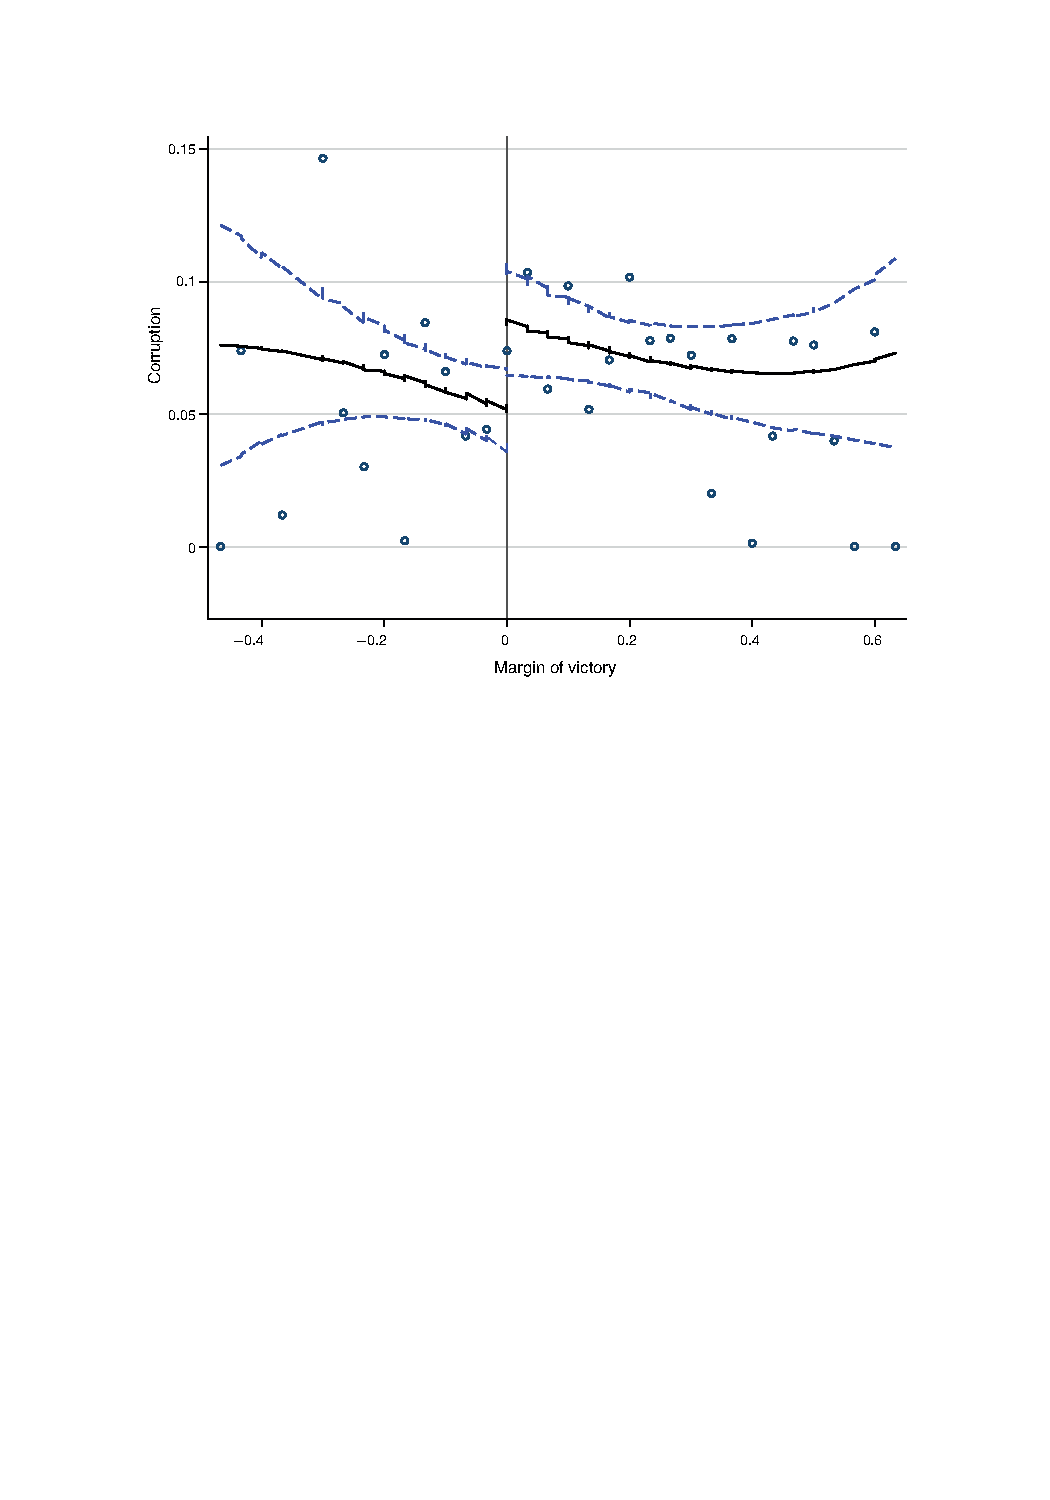
\includegraphics[scale=.75]{FigureRDD.pdf}
\end{center}
\end{figure}
}


\end{document}
